\documentclass[conference]{IEEEtran}
\IEEEoverridecommandlockouts
% The preceding line is only needed to identify funding in the first footnote. If that is unneeded, please comment it out.
\usepackage{cite}
\usepackage{amsmath,amssymb,amsfonts}
\usepackage{algorithmic}
\usepackage{graphicx}
\usepackage{textcomp}
\usepackage{xcolor}
\usepackage{graphicx}
\usepackage[colorlinks=true,citecolor=blue]{hyperref}
\def\BibTeX{{\rm B\kern-.05em{\sc i\kern-.025em b}\kern-.08em
    T\kern-.1667em\lower.7ex\hbox{E}\kern-.125emX}}
\usepackage{enumitem}
\usepackage{lipsum} % für Beispieltext

% Stildefinition
\newlist{myitemize}{itemize}{1}
\setlist[myitemize]{%
  label=\textbullet,
  leftmargin=*,
  itemsep=0pt,
  parsep=0pt,
  listparindent=1.5em, % Einrückung der ersten Zeile eines Absatzes
}

\begin{document}

\title{Untersuchung der Nachweisbarkeit des Akkommodation-Vergenzkonflikts in einem EEG in einer VR entspannungs Szene\\
\thanks{HFU Furtwangen}
}

\author{
	\IEEEauthorblockN{Nick Philipp Häcker}
	\IEEEauthorblockA{\textit{Fakultät Digitale Medien} \\
	\textit{Hochschule Furtwangen}\\
	Furtwangen, Deutschland \\
	haeckern@hs-furtwangen.de}
	
	\and
	\IEEEauthorblockN{Suzan Johannes}
	\IEEEauthorblockA{\textit{Fakultät Digitale Medien} \\
	\textit{Hochschule Furtwangen}\\
	Furtwangen, Deutschland \\
	s.johannes@hs-furtwangen.de}
	\and
	
	\IEEEauthorblockN{Patrick Kaserer}
	\IEEEauthorblockA{\textit{Fakultät Digitale Medien} \\
	\textit{Hochschule Furtwangen}\\
	Furtwangen, Deutschland \\
	patrick.kaserer@hs-furtwangen.de}
	\and
	
	\IEEEauthorblockN{Johann Schulenburg}
	\IEEEauthorblockA{\textit{Fakultät Digitale Medien} \\
	\textit{Hochschule Furtwangen}\\
	Furtwangen, Deutschland \\
	johann.schulenburg@hs-furtwangen.de}
	
	\and
	\IEEEauthorblockN{Lukas Willmann}
	\IEEEauthorblockA{\textit{Fakultät Digitale Medien} \\
	\textit{Hochschule Furtwangen}\\
	Furtwangen, Deutschland \\
	Lukas.willmann@hs-furtwangen.de}
}

\maketitle

\begin{abstract}
This document is a model and instructions for \LaTeX.
This and the IEEEtran.cls file define the components of your paper [title, text, heads, etc.]. *CRITICAL: Do Not Use Symbols, Special Characters, Footnotes, 
or Math in Paper Title or Abstract.
\end{abstract}

\begin{IEEEkeywords}
virtual reality, akkommodation-vergenz konflikt, elektroenzephalografie
\end{IEEEkeywords}

\section{Einleitung}
“Applications of Computer Science, including digital games, virtual reality, and augmented reality [...], have enormous potential for bringing about cultural change.”\cite{b2}\\
VR-Brillen verwenden Stereoskopie, bei der jedem Auge durch eine horizontale Verschiebung der Bilder leicht unterschiedliche Informationen zugeführt werden. So entsteht beim Nutzer eine 3D-Wirkung der Darstellung. Durch die negativen Parallaxen kann die Szene den Eindruck erwecken, aus der Leinwand hervorzutreten oder dahinter zu liegen.\cite{b3}\\
Die vorliegende Untersuchung konzentriert sich auf den Akkommodation-Vergenz-Konflikt. Dieser tritt insbesondere in der modernen VR-Technologie auf, da durch die Linsen der VR-Brille die Bildebene in eine weite Entfernung projiziert wird, während die Objekte in der VR durch Interaktion in greifbarer Nähe erscheinen.
“In order to see one object, the eyeballs need to rotate accordingly. This mechanism is called the “vergence”. In a natural situation, as an object is moving closer or further, vergence matches another physiological phenomena: “accommodation”. It enables the object’s image to remain clear on the retina. It is caused by a deformation of the crystalline lens, which focuses light beams the same way camera lenses do.”\cite{b4}

Einige Hirnregionen, insbesondere das Mittelhirn, sind hinsichtlich der Okulomotorik besonders relevant. Aus dem Mittelhirn verlaufen drei Hirnnerven zu den Augen, wobei der N. oculomotorius unter anderem auch für die Akkommodation des Auges verantwortlich ist \cite{b5}. Eine besondere Herausforderung ist die Bestimmung, ob die gemessenen EEG-Werte tatsächlich auf den Akkommodation-Vergenz-Konflikt zurückzuführen sind. Denn während des Sehvorgangs werden verschiedene Gehirnregionen aktiviert, darunter die primäre Sehrinde im hinteren Hauptlappen der Großhirnrinde, der Scheitellappen zur Lokalisierung von Objekten und der Schläfenlappen zur Objekterkennung \cite{b6}. Letztlich könnte der primäre sensorische Kortex, insbesondere die von Wilder Penfield identifizierten Bereiche, durch starke Werte aufzeigen, ob der Akkommodation-Vergenz-Konflikt im EEG nachweisbar ist \cite{b7}.

Ziel dieser Untersuchung ist es zu ermitteln, ob mögliche Probleme in Anwendungen, die im kritischen Bereich des Akkommodations-Vergenz-Konflikts arbeiten, mittels EEG nachweisbar sind. Damit könnte zukünftige Forschung gezielter auf diesen Bereich ausgerichtet werden \cite{b8}.\\
Dieses Forschungsgebiet ist von großer Bedeutung, da VR-Technoligien zunehmend in verschiendenen Bereichen wie Gaming, Bildung, Gesundheitswesen und Industrie eingesetzt werden und ein besseres Verständnis des Akkommodation-Vergenz-Konflikt dazu beitragen kann, die zukünftige Entwicklung von VR-Anwendungen zu verbessern.

\section{Related Work}
\subsection{Assessing the zone of comfort in stereoscopic displays using EEG}
In ihrem Paper "Assessing the zone of comfort in stereoscopic displays using EEG" \cite{b1} untersuchten die Autoren, wie der Akkommodations-Vergenz-Konflikt bei stereoskopischen Darstellungen die EEG-Aktivität beeinflusst. Ihr Ziel war die Entwicklung eines adaptiven Systems, das mithilfe von tragbaren EEG-Geräten die Darstellung individuell für jeden Betrachter kalibrieren kann, um unangenehme Erfahrungen zu vermeiden.

Eine Pilotstudie wurde durchgeführt, bei der kurze Betrachtungssequenzen verwendet wurden, um Ergebnisse innerhalb eines kurzen Zeitraums zu erzielen, bevor sich die Probanden an die Darstellung gewöhnen konnten. Der experimentelle Aufbau bestand darin, den Probanden einen Meter vor einen Bildschirm zu setzen. Zunächst wurde eine Szene von 2-5 Sekunden gezeigt, in der ein Würfel in Null-Parallaxe auf dem Bildschirm dargestellt wurde. Anschließend wurde er zufällig in eine von neun Positionen versetzt und für 5 Sekunden stereoskopisch vor oder hinter dem Bildschirm dargestellt. Diese Positionen variierten in einer Entfernung von 0,212 m bis 3,046 m vom Probanden und wurden als komfortabel (C) oder unkomfortabel (NC) eingestuft. Nach den fünf Sekunden musste der Proband angeben, ob er den Würfel vor oder hinter dem Bildschirm wahrnahm. Dieser Versuch wurde sowohl nur mit Fragebogen als auch in Kombination mit EEG-Messung und Fragebogen durchgeführt. Bei der EEG-Messung nahmen drei Probanden teil.
 
In der Analyse der ereignisbezogenen Potenziale (ERP) ergaben sich Unterschiede zwischen den Bedingungen Komfort (C) und Unkomfort (NC). In der Unkomfort-Bedingung war die positive Komponente im ERP verzögert, während die negative Komponente in der Komfort-Bedingung eine höhere Amplitude aufwies. Die Untersuchung der Frequenzbänder (ERSP) zeigte ebenfalls Unterschiede zwischen den Bedingungen Komfort und Unkomfort. In der Unkomfort-Bedingung wurde eine Abnahme der Aktivität im Alpha-Band (10-14 Hz) festgestellt, während eine Zunahme der Aktivität im Theta-Band (4-7 Hz) und Beta-Band (15-25 Hz) im Vergleich zur Komfort-Bedingung beobachtet wurde. Die Probanden schnitten in der unkomfortablen Bedingung besser bei der Tiefenwahrnehmung ab. Die Ergebnisse des Fragebogens ergaben, dass klares Unwohlsein durch die visuelle Darstellung ausgelöst wurde. Es wurden Widersprüche zu früheren Studien festgestellt, die Stereoskopie mit 2D-Bildern verglichen haben. Es wurden Verbesserungen vorgeschlagen, wie die Messung des Pupillenabstands und die Verwendung fortschrittlicherer Technologien wie VR-Brillen. Die Autoren vermuten, dass die EEG-Messung nicht nur zur Optimierung der Stereoskopie dienen kann, sondern auch zur Entwicklung von Leitlinien für eine verbesserte Technologie.

In unserem Versuch können wir unsere EEG-Ergebnisse mit den Ergebnissen dieser Studie in Bezug auf die EEG-Ergebnisse vergleichen. Hervorzuheben sind jedoch Unterschiede, wie zum Beispiel, dass die 3D-Szene in unserem Experiment deutlich komplexer ist als der Aufbau in dieser Studie. Ebenfalls wichtig ist die Anzahl der Versuchspersonen und die Tatsache, dass in unserem Versuch eine konstante Veränderung der Position des Würfels durchgeführt wurde und nicht zu jeder Position der Sehkomfort abgefragt wurde. Bezüglich des technischen Aufbaus ist zu berücksichtigen, dass in unserem Versuch beim Einrichten der VR-Brille der Pupillenabstand der Probanden beachtet wurde und mit der VR-Brille ein deutlich immersiveres Medium verwendet wurde als ein 3D-Bildschirm.


\subsection{Study of Electroencephalography-based Objective Stereoscopic Visual Fatigue Evaluation}
In der Studie "Untersuchung der elektroenzephalographiebasierten objektiven stereoskopischen visuellen Ermüdungsbewertung" \cite{b5} wird der Zusammenhang zwischen visueller Ermüdung durch den Akkommodations-Vergenz-Konflikt bei 3D-Displays mittels EEG-Messung hergestellt.
Das Experiment wurde mit 11 Studenten durchgeführt. Sie wurden gebeten, auf einem Random Dot Stereogramm festzustellen, in welche Richtung ein abgebildeter Pfeil zeigt. Es gab eine Übungszeit von fünf Minuten, gefolgt von sieben Testläufen à zehn Minuten.
Die Forscher konnten einen stärkeren Anstieg der Alpha-Wellen im Frontalbereich des Gehirns über die Dauer des Experiments feststellen. Die Aktivität der Beta-Wellen stieg ebenfalls an, jedoch nicht so stark wie die der Alpha-Wellen. Die Forscher stellten fest, dass die Art der Aufgabe auch Einfluss auf die Aktivitäten der Wellen haben könnte. Sie schlussfolgern, dass ihr Befund der erhöhten Alpha-Wellen-Aktivität im Frontallappen ein Indikator für visuelle Ermüdung sein könnte.
Auch hier können die EEG-Ergebnisse mit unseren Ergebnissen verglichen werden. Aufgrund der Beschreibung des Versuchsaufbaus ist jedoch unklar, wie stark der Akkommodations-Vergenz-Konflikt in diesem Experiment ausgelöst wurde. Es ist auch zu beachten, dass ein Random Dot Stereogramm auf einem 3D-Display sehr unterschiedliche Ergebnisse liefern kann im Vergleich zu einer komplexen 3D-Szene auf einem VR-Headset.
 

\section{Methodik}
\subsection{Material}
Für das Experiment wurde eine Vive Pro VR-Brille \cite{b11} eingesetzt. Die EEG-Messung wurde mit dem DSI-24 von Neurospec durchgeführt, einem Einem Dry Sensor Interface \cite{b9}. Für die Erfassung der Antworten im SSQ und der allgemeinen Daten wurden die Fragebögen mit Google Forms erstellt. Um den Datenschutz zu gewährleisten, wurden zur Zuordnung der Daten anonyme Codes verwendet und es wurden keine personenbezogenen Daten der Teilnehmer online gespeichert. Die Auswertung der EEG-Daten erfolgte mit der Software "BESA Research" von BESA \cite{b10}. Die Entspannungsszene, in der sich der Teilnehmer während des Experiments befand, wurde von einer vorherigen Forschungsgruppe in Unity entwickelt. Diese konnte Ergebnisse erzielen, die auf eine positive Wirkung auf die Entspannung der Nutzer hinweisen. Anpassungen für dieses Experiment und die Durchführung des Experiments wurden ebenfalls in Unity vorgenommen.

\subsection{Versuchsdurchführung}
Das Experiment wurde in den Räumlichkeiten der Hochschule Furtwangen durchgeführt. Vor Beginn des Tests wurden die Probanden nach bekannten Sehschwächen, Epilepsie oder bestehender partieller Blindheit befragt. Nachdem die Teilnehmer die Einverständniserklärung zur Datenverarbeitung und Risiken akzeptiert hatten, wurde ein Random-Dot-Test zur Erfassung des möglichen Tiefensehens durchgeführt und der interpupillare Abstand (IPD) gemessen. Anschließend füllten die Probanden einen Pre-Simulator-Sickness-Fragebogen aus. Nach dem Ausfüllen des Fragebogens wurden sie auf einen Liegestuhl gebeten. Hier wurde die VR-Brille entsprechend der gemessenen IPD eingestellt und das EEG aufgesetzt. Den Probanden wurde mitgeteilt, dass sie während des Tests starkes Zwinkern, bewusste Kopfbewegungen oder Zähneknirschen vermeiden sollten, da diese Faktoren die EEG-Messdaten beeinflussen können.

Nachdem alle Geräte angelegt und kalibriert waren, wurde den Probanden eine Entspannungsszene vorgeführt. In dieser Szene war ein Würfel mit einem grünen Punkt auf seiner Oberfläche zu sehen. Diese Markierung sollte das Fokussieren des Würfels erleichtern. Nachdem der Proband mit einer Handbewegung signalisiert hatte, dass er sich in der Szene wohl fühlte, bewegte sich der Würfel langsam auf ihn zu. Der Proband sollte während dieser Phase kontinuierlich den Würfel fokussieren. Innerhalb von vier Minuten legte der Würfel in der VR eine Strecke von etwa 13 Metern zurück und stoppte in einer Entfernung von 13 Zentimetern zum Probanden. Nach einer Verweildauer von zehn Sekunden in dieser Position füllte der Proband den Post-Simulator-Sickness-Fragebogen aus.

Der Stimuli des Tests ist der Würfel, welcher sich dem Probanden durchgehend in den 4 Minuten in einer konstanten Geschwindigkeit nähert. Um das Erkennen der genauen Entfernung des Würfels für den Probanden zu verhindern wurde der Würfel in seiner Skalierung verhältnismäßig zur Entfernung zum Probanden kleiner Skaliert (…f*Scale/distance… richtige Formel einfügen). Durch die Entfernung dieser monokularen Tiefeninformation soll das Annähern des Würfels eine mögliche bedrohliche Wirkung auf den Probanden verringern. In der Szene wurde ein Bereich gewählt in welchem möglichst wenig Bäume  vorhanden sind, damit es beim Probanden nicht zu Problemen der Fixationsdisparitäten kommt.

Die Durchführung des Experiments dauerte insgesamt etwa 25 bis 50 Minuten. Sieben bis zehn Minuten davon wurden für die Einführung und die Fragebögen benötigt, fünf Minuten für die Zeit in der VR und etwa 10 bis 35 Minuten für das Anlegen und Kalibrieren des EEGs. 

\subsection{Datenerhebung und Verarbeitung}
Die mit Google Forms gesammelten Daten konnten als CSV-Dateien heruntergeladen werden. Diese Daten wurden dann in Excel weiterverarbeitet. Die demografischen Daten wurden als Kreisdiagramme (Fig 2) und Boxplots dargestellt (Fig 1).\\
Die Ergebnisse des Simulator-Sickness-Fragebogens (SSQ) wurden im Vorher-Nachher-Vergleich als Boxplots gegenübergestellt (Fig 3).\\
Um eine mögliche Signifikanz der Vorher- und Nachher Ergebnisse der SSQ Ergebnisse zu ermitteln wurde in Excel ein einseitiger t-Test durchgeführt.\\ 
!! Nick hier seinen Teil !!

\section{Ergebnisse}
Durch die t-Test Analyse konnten keine signifikanten Ergebnisse bei allen Indikatoren des SSQ-Tests ermittelt werden. Die Nullhypothese, dass die Durchführung in der VR-Szene des Tests zu Simulator-Sickness führt musste nicht verworfen werden. Bei einem Alpha = 0.05 wurden die geringsten Werte bei Schwitzen (p = 0,052) und Erhöhter Speichelfluss (p = 0,082) festgestellt werden.\\
\begin{figure}[ht]
	\centering
	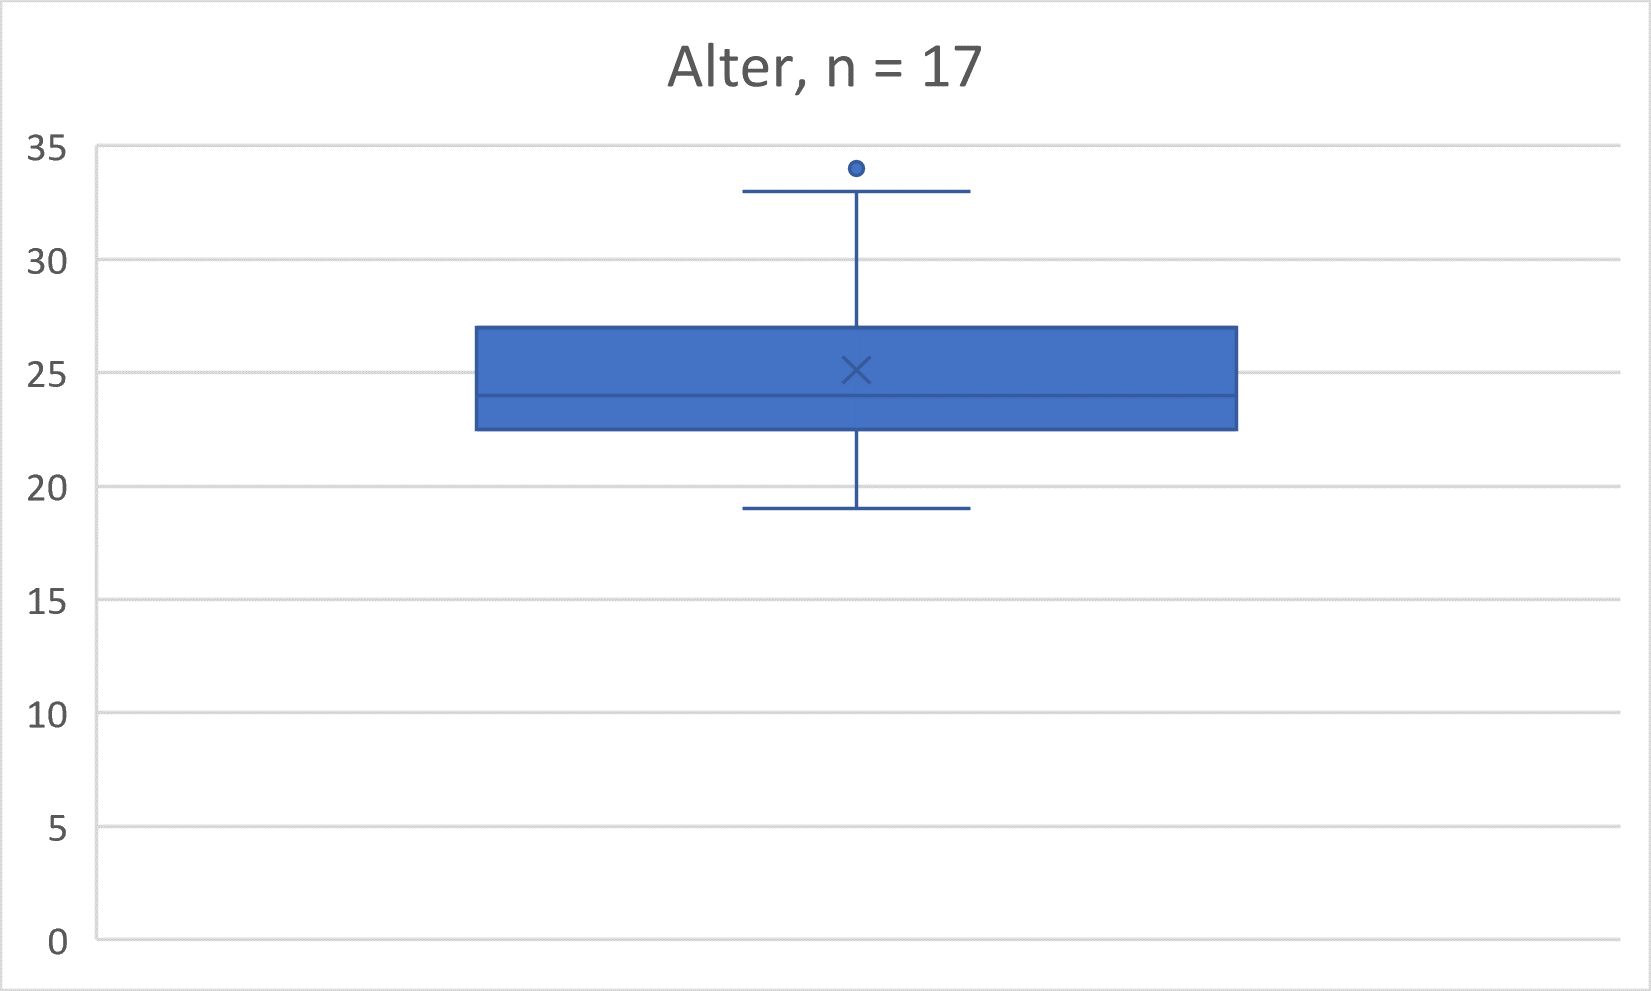
\includegraphics[width=0.2\textwidth]{assets/alter.png} \hspace{-5pt}
	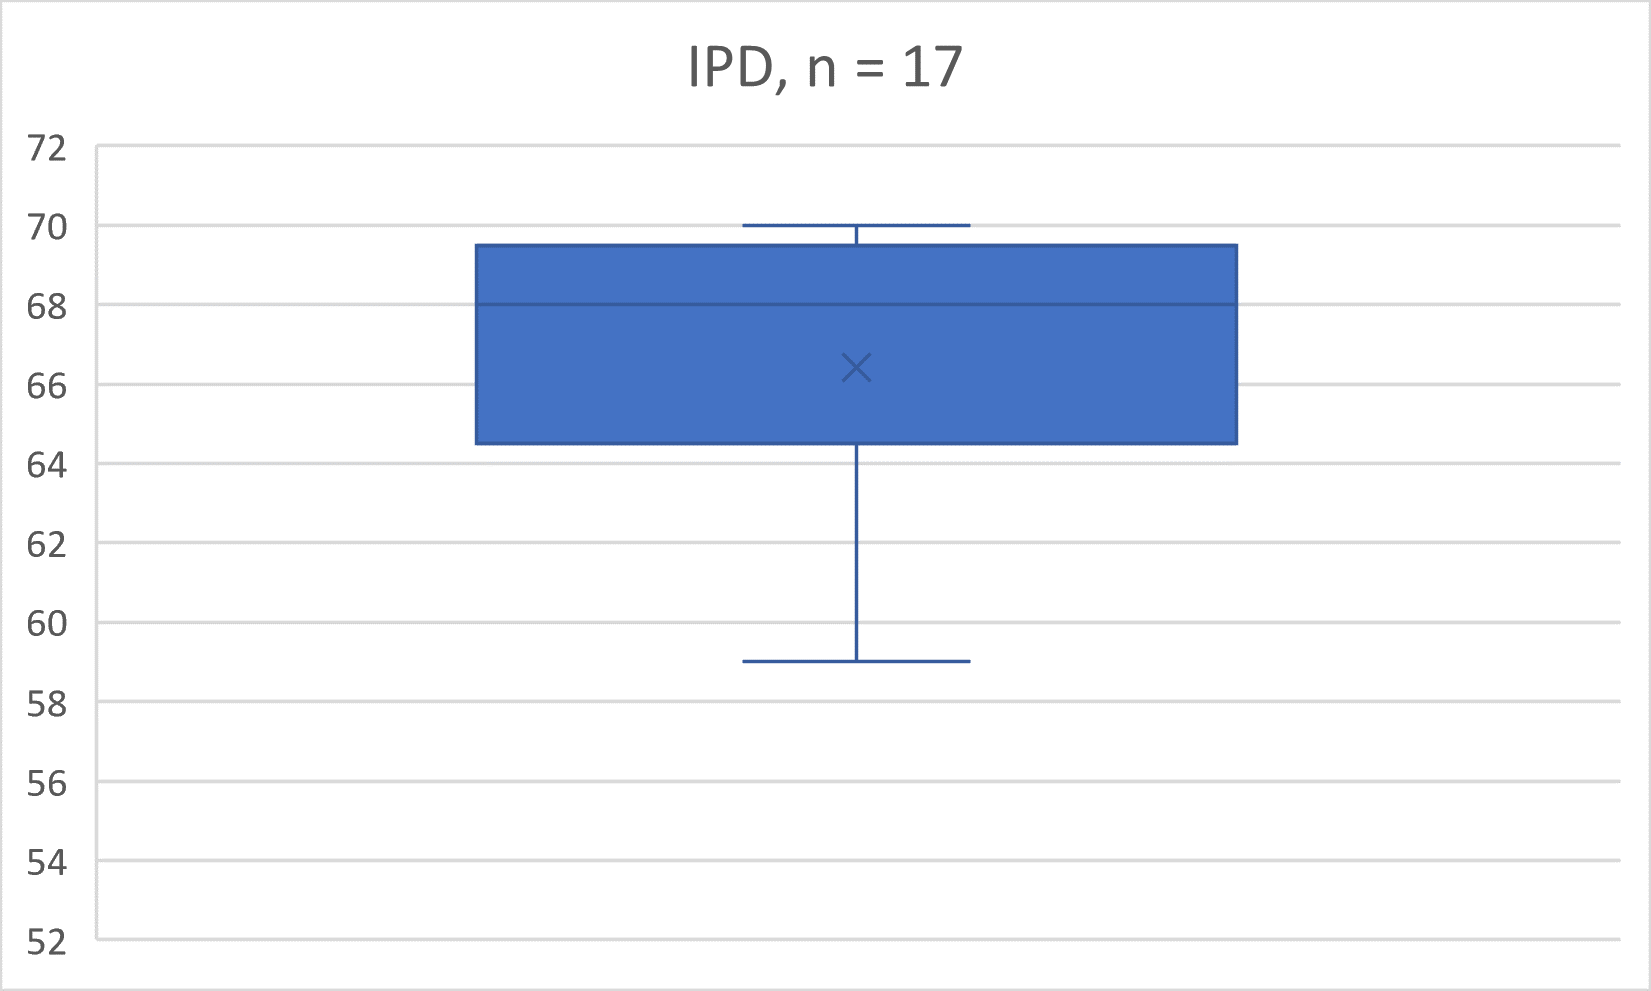
\includegraphics[width=0.2\textwidth]{assets/ipd.png} \\
	\vspace{2pt}
	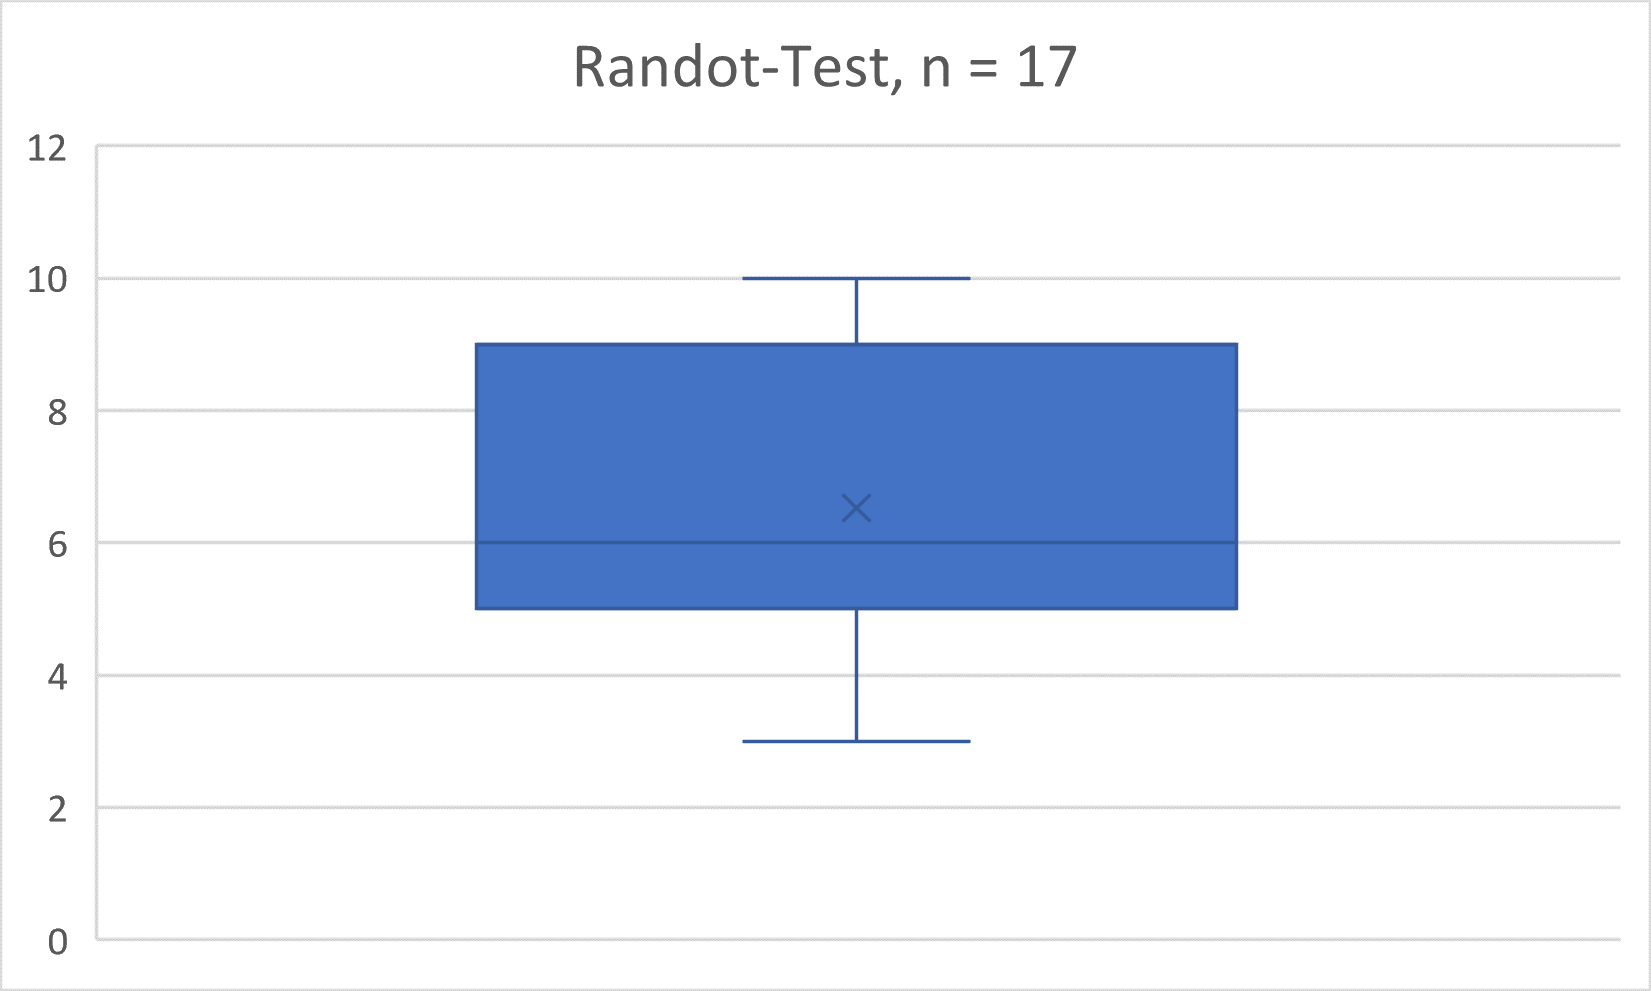
\includegraphics[width=0.2\textwidth]{assets/randot.png} \hspace{-5pt}
	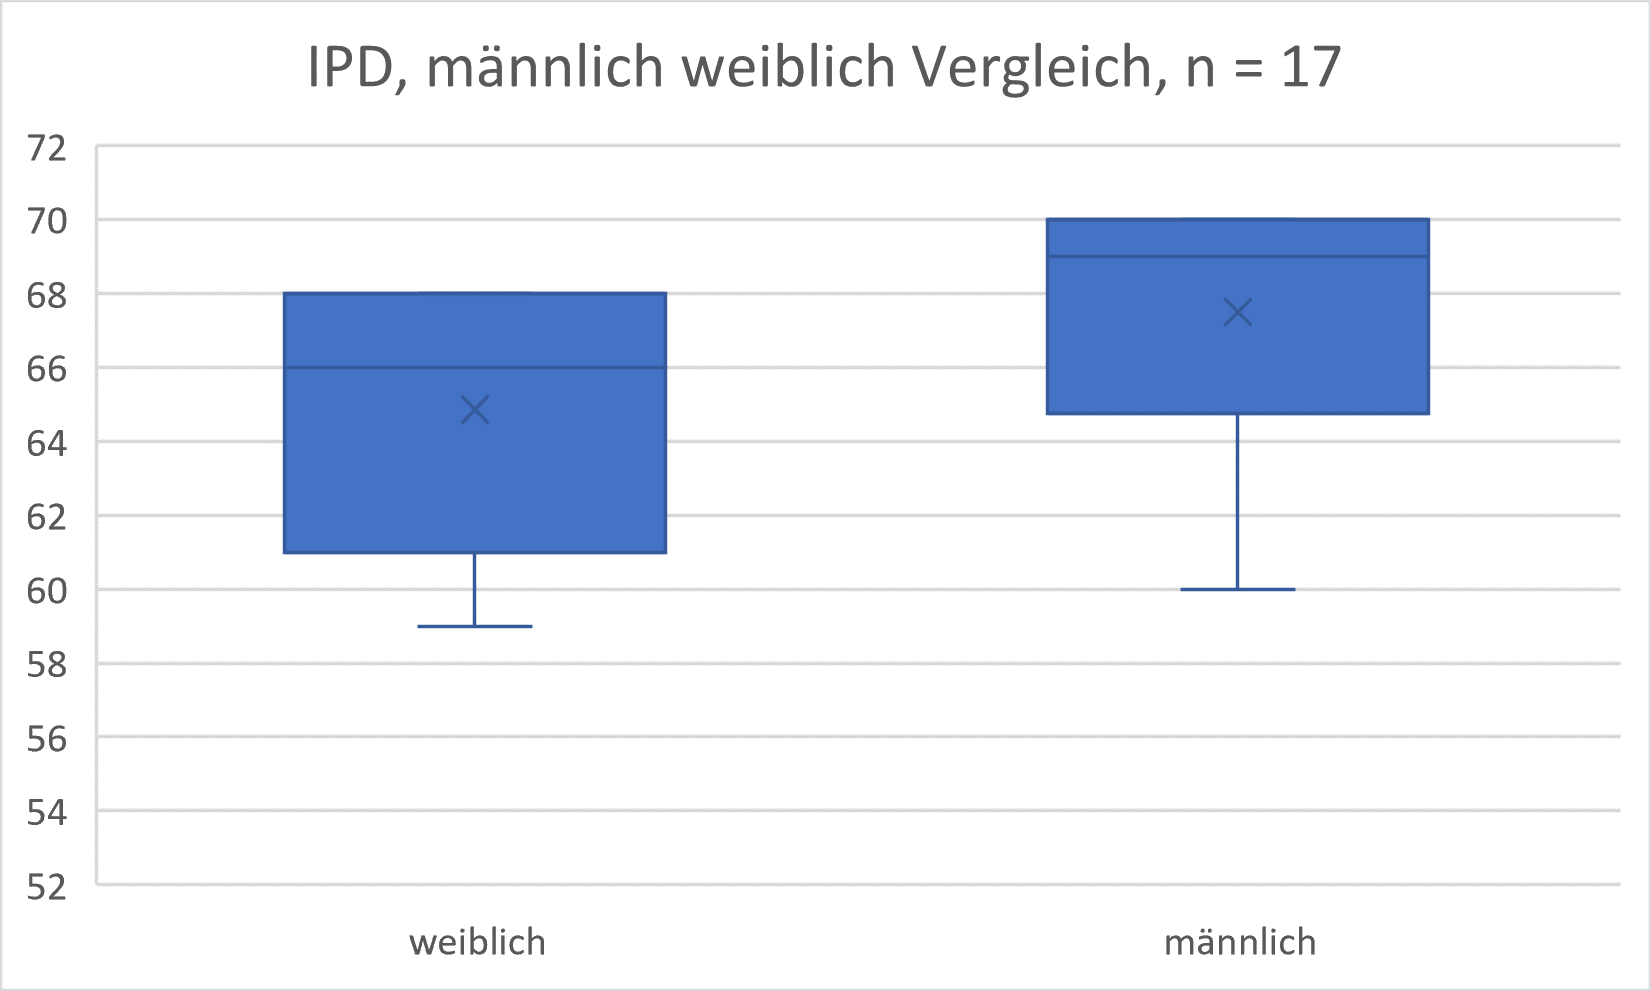
\includegraphics[width=0.2\textwidth]{assets/ipd_mvw.png}\\
	\caption{Demografische Daten}
	\label{fig:Demografische Daten}
\end{figure}
Lorem ipsum dolor sit amet, consetetur sadipscing elitr, sed diam nonumy eirmod tempor invidunt ut labore et dolore magna aliquyam erat, sed diam voluptua. At vero eos et accusam et justo duo dolores et ea rebum. Stet clita kasd gubergren, no sea takimata sanctus est Lorem ipsum dolor sit amet. Lorem ipsum dolor sit amet, consetetur sadipscing elitr, sed diam nonumy eirmod tempor invidunt ut labore et dolore magna aliquyam erat, sed diam voluptua. At vero eos et accusam et justo duo dolores et ea rebum. Stet clita kasd gubergren, no sea takimata sanctus est Lorem ipsum dolor sit amet.

\begin{figure}[ht]
	\centering
	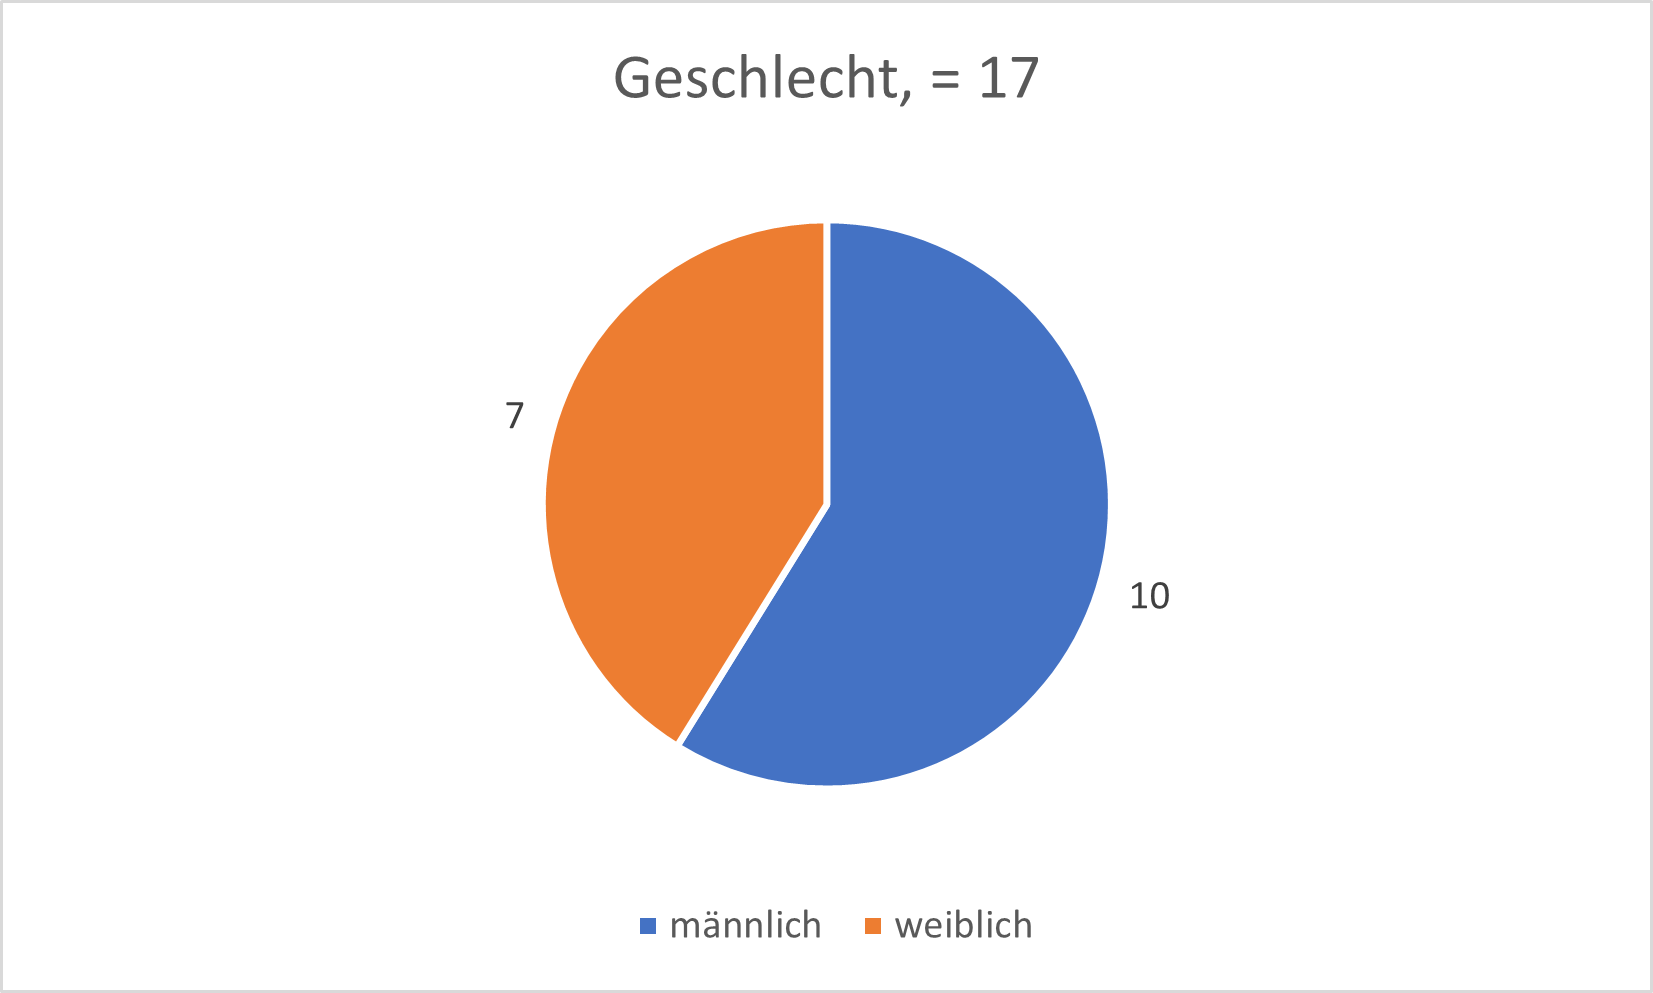
\includegraphics[width=0.2\textwidth]{assets/gesch.png} \hspace{-5pt}
	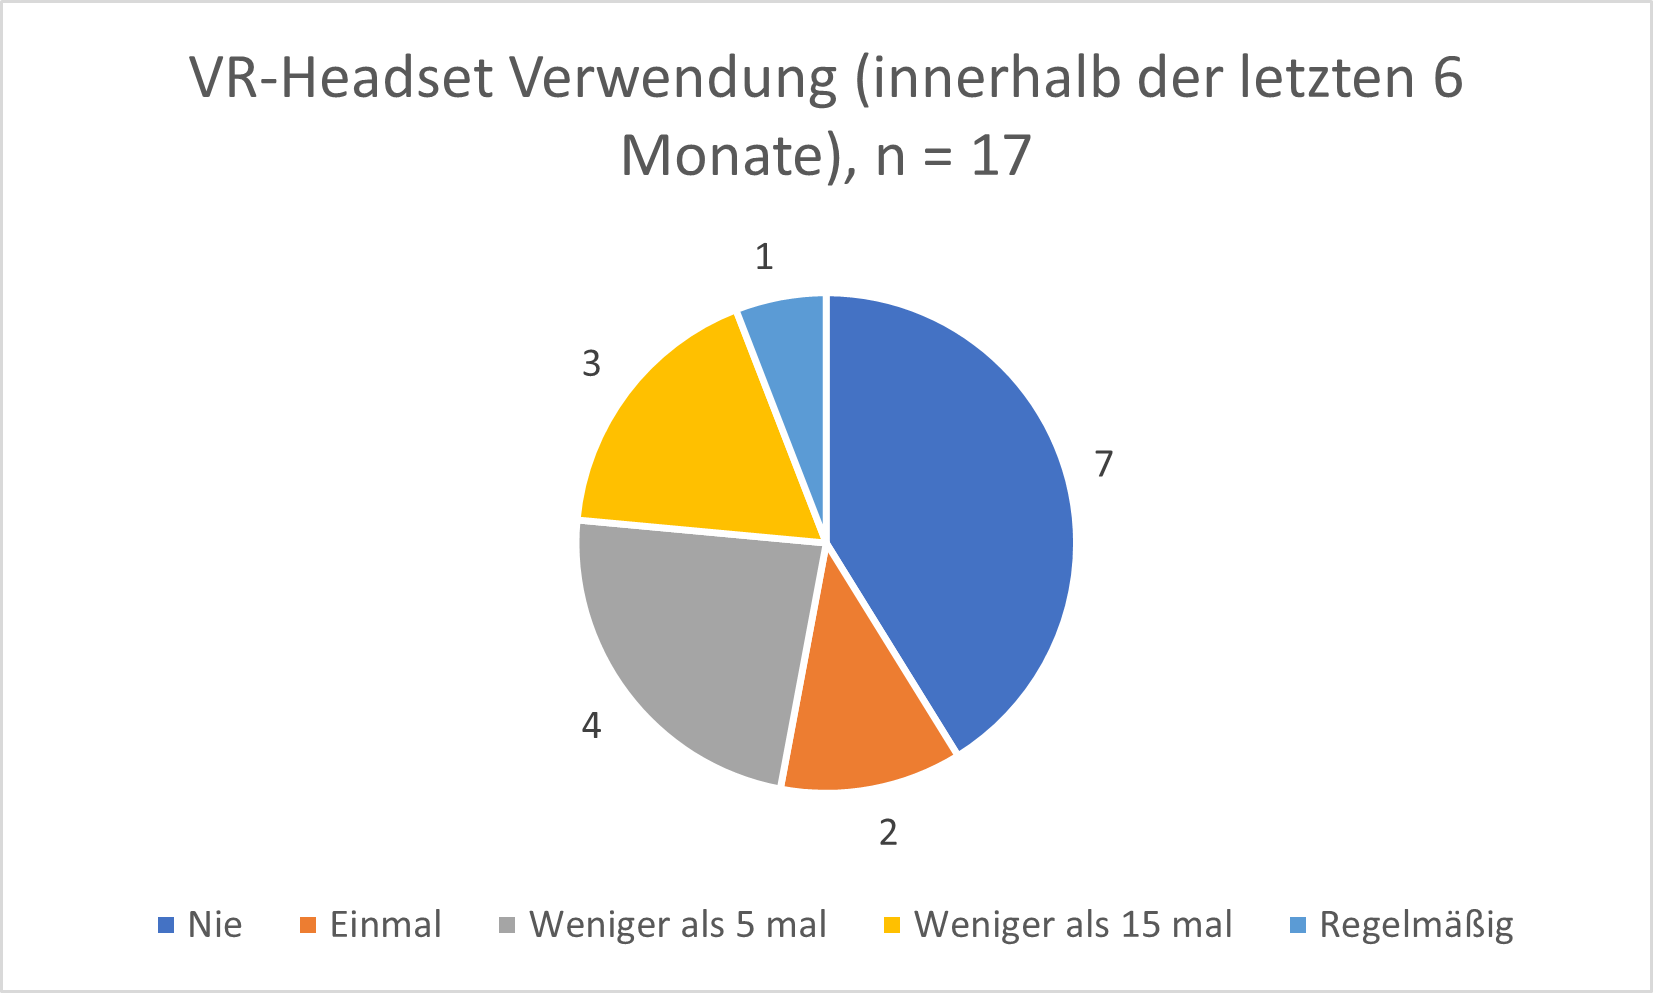
\includegraphics[width=0.2\textwidth]{assets/headset.png} \\
	\vspace{2pt}
	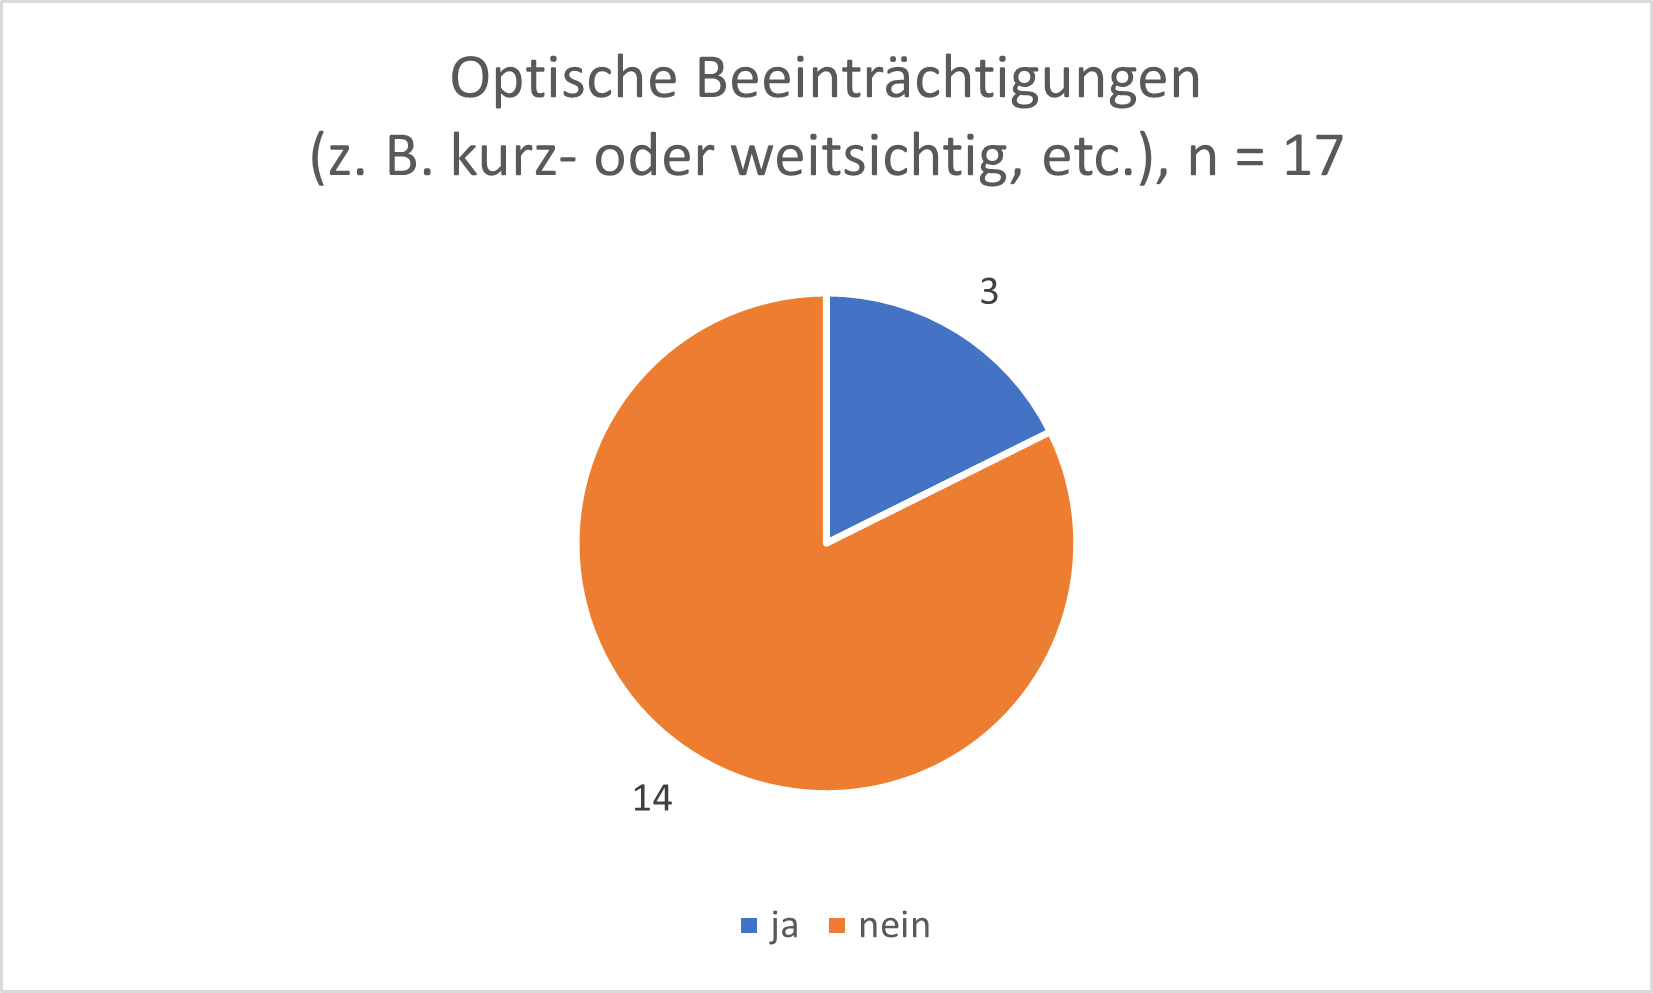
\includegraphics[width=0.2\textwidth]{assets/optBeein.png} 
	\caption{Demografische Daten 2}
	\label{fig:Demografische Daten 2}
\end{figure}
Lorem ipsum dolor sit amet, consetetur sadipscing elitr, sed diam nonumy eirmod tempor invidunt ut labore et dolore magna aliquyam erat, sed diam voluptua. At vero eos et accusam et justo duo dolores et ea rebum. Stet clita kasd gubergren, no sea takimata sanctus est Lorem ipsum dolor sit amet. Lorem ipsum dolor sit amet, consetetur sadipscing elitr, sed diam nonumy eirmod tempor invidunt ut labore et dolore magna aliquyam erat, sed diam voluptua. At vero eos et accusam et justo duo dolores et ea rebum. Stet clita kasd gubergren, no sea takimata sanctus est Lorem ipsum dolor sit amet.

\begin{figure}[ht]
	\centering
	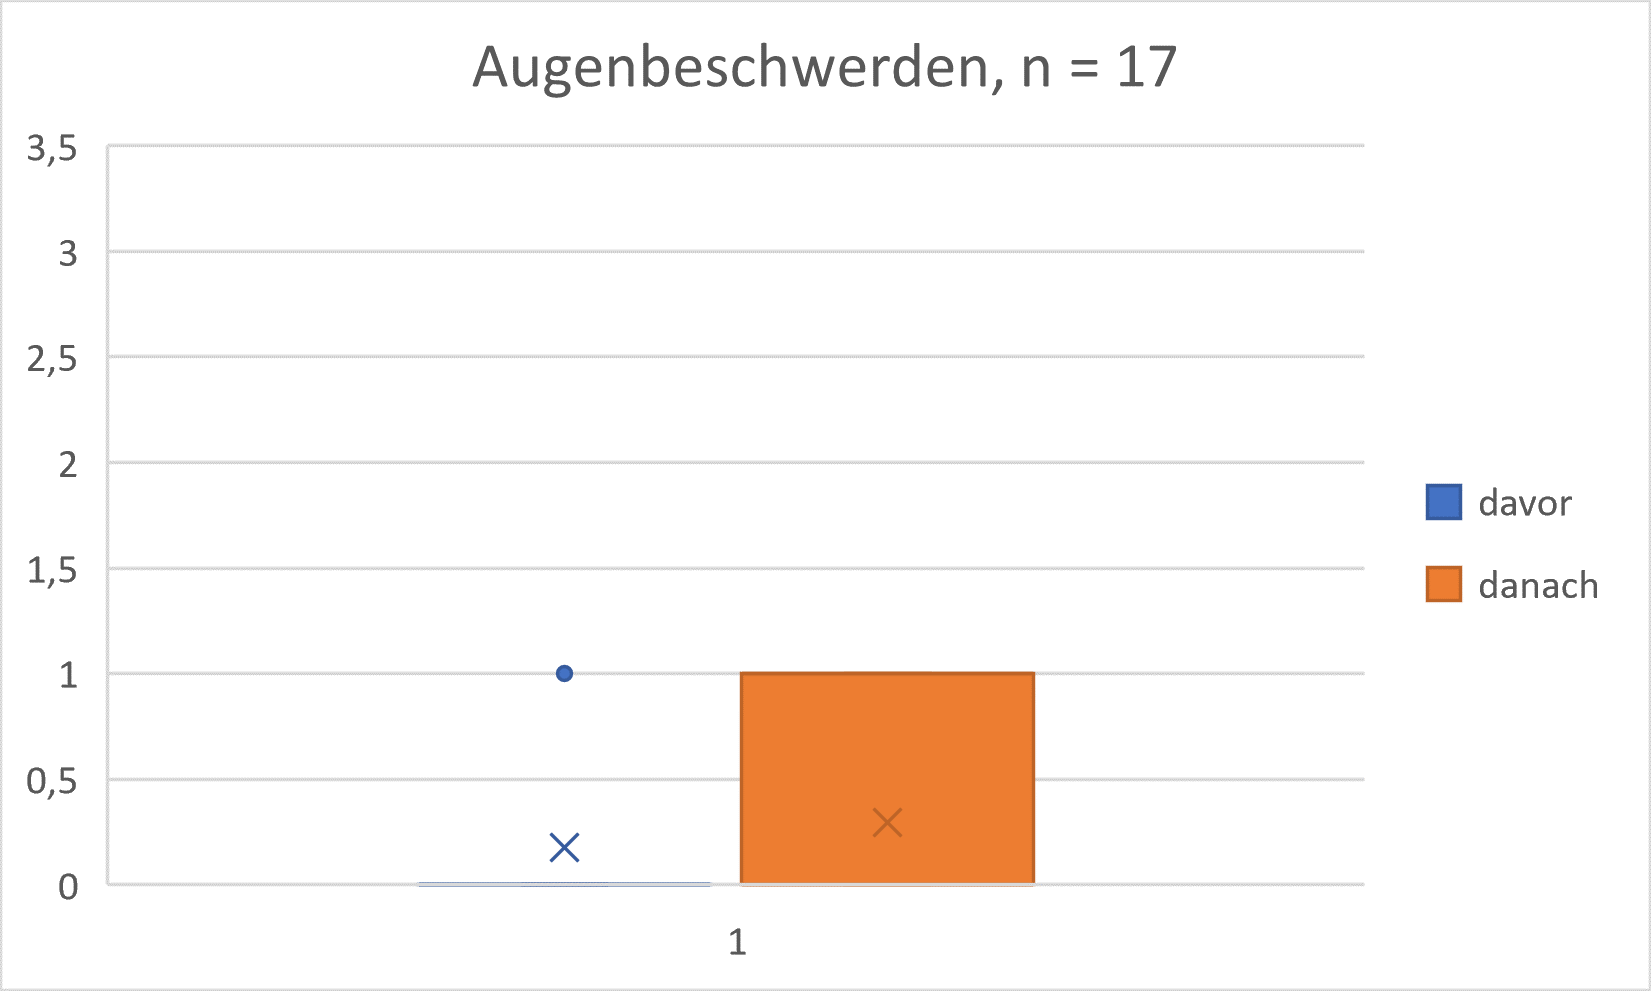
\includegraphics[width=0.2\textwidth]{assets/augenBesch.png} \hspace{-5pt}
	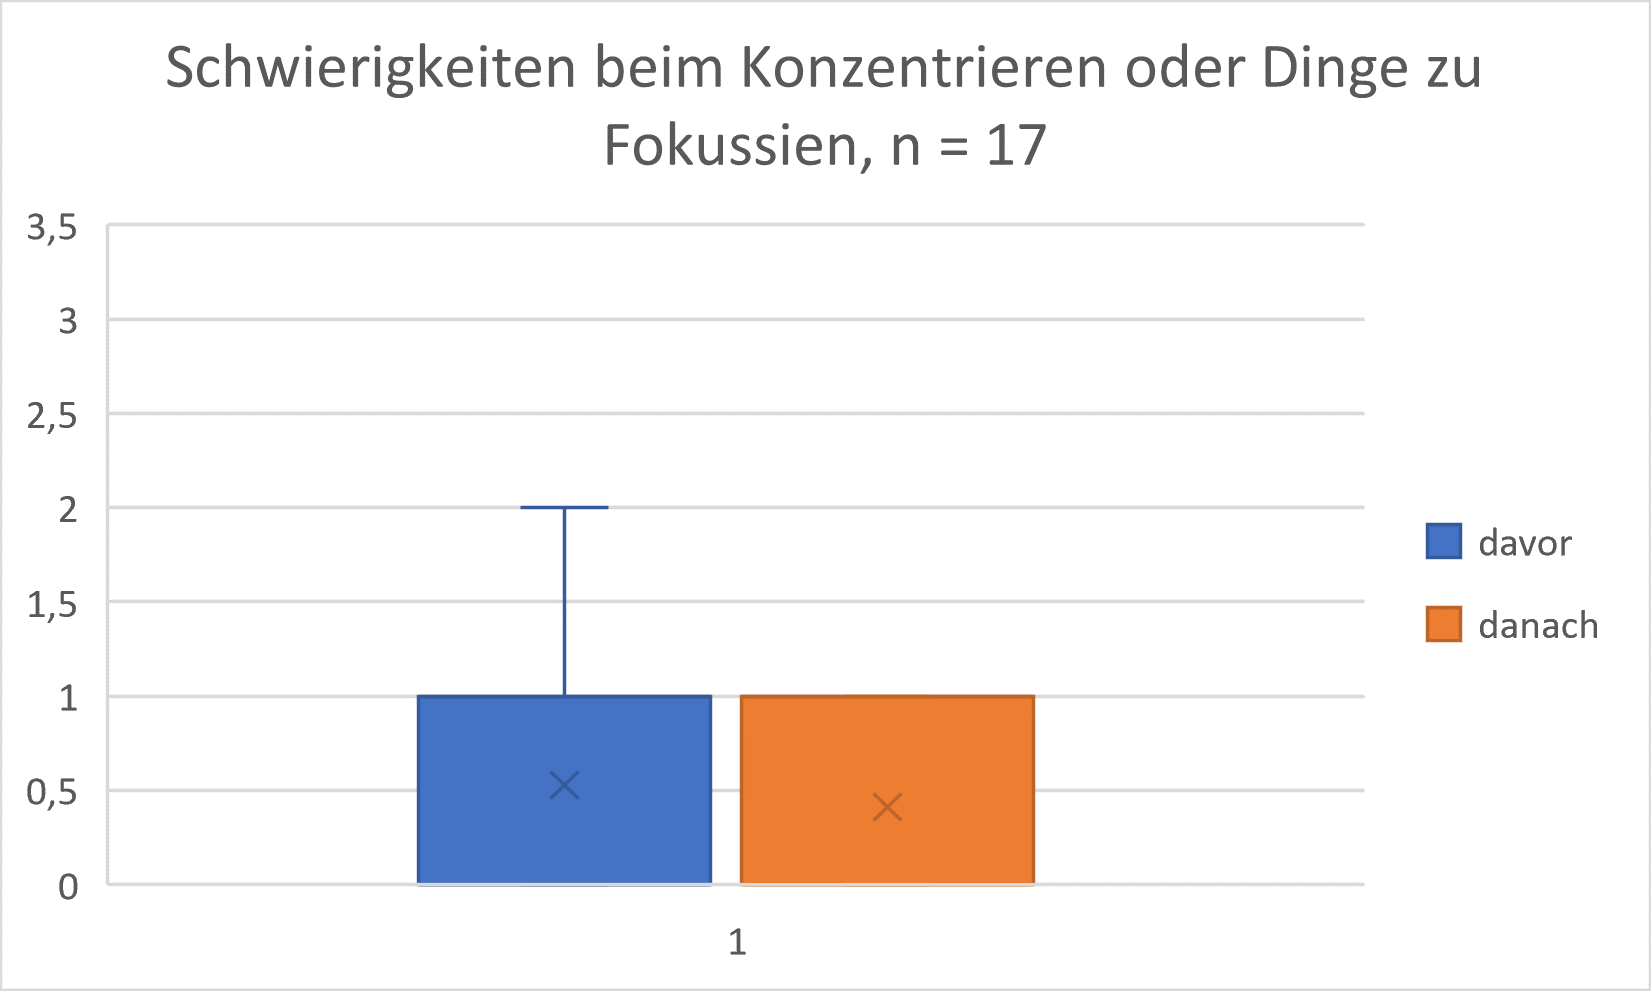
\includegraphics[width=0.2\textwidth]{assets/fokus.png} \\
	\vspace{2pt}
	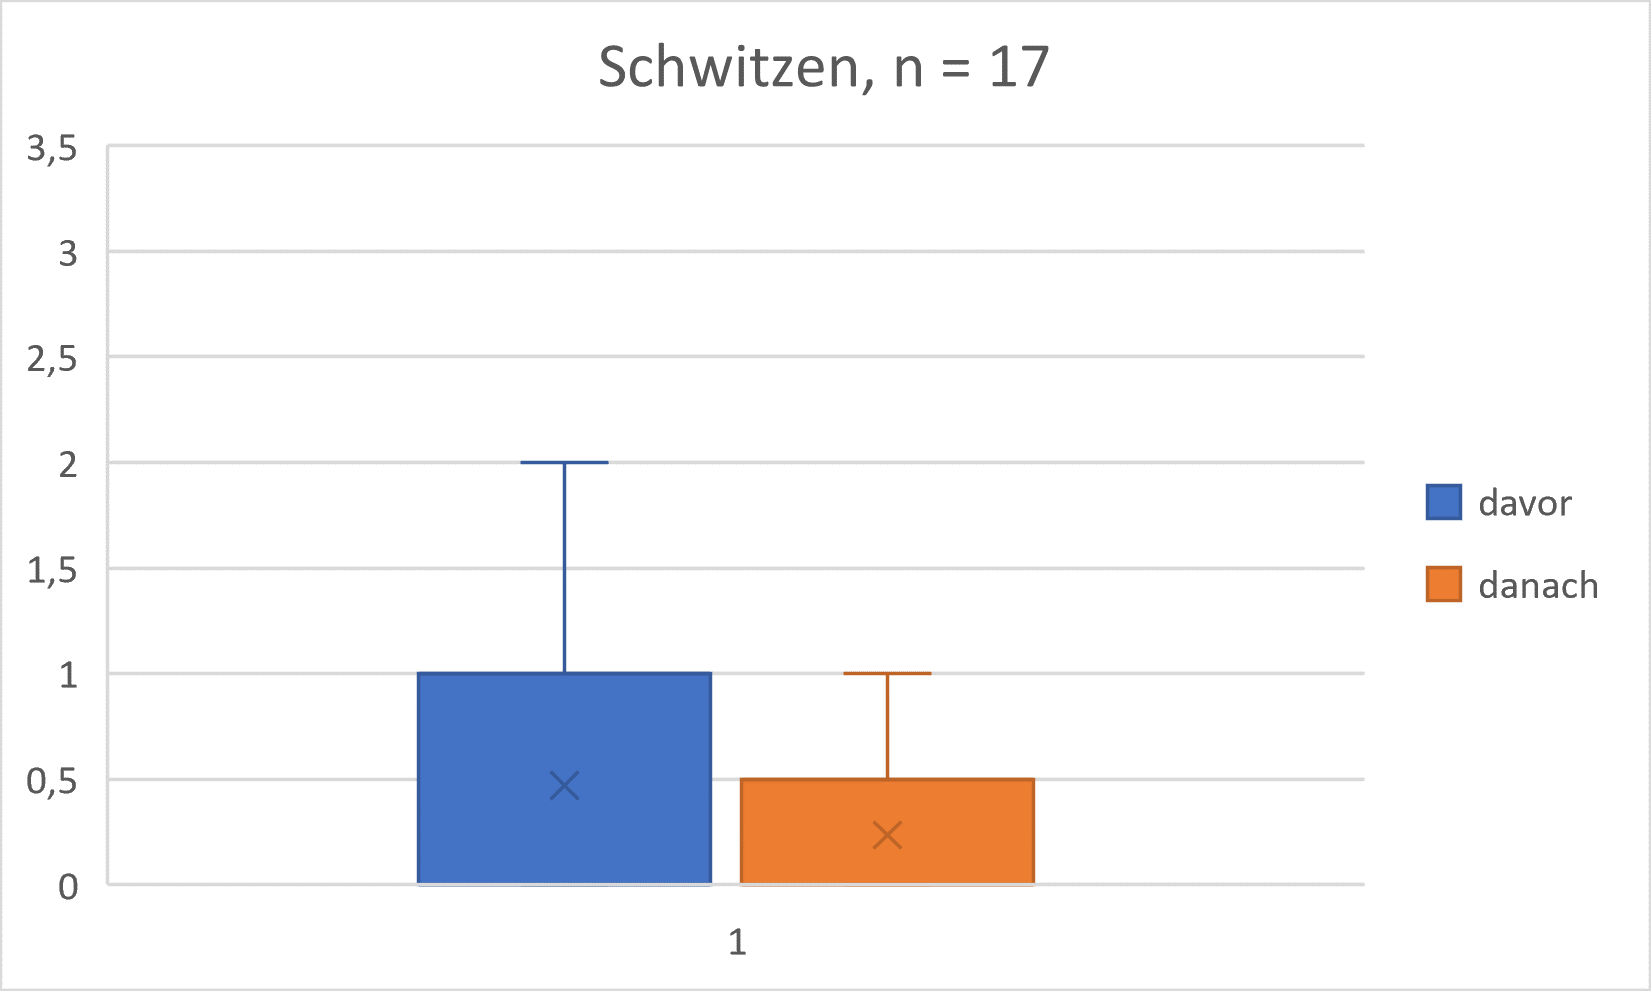
\includegraphics[width=0.2\textwidth]{assets/schwitz.png} \hspace{-5pt}
	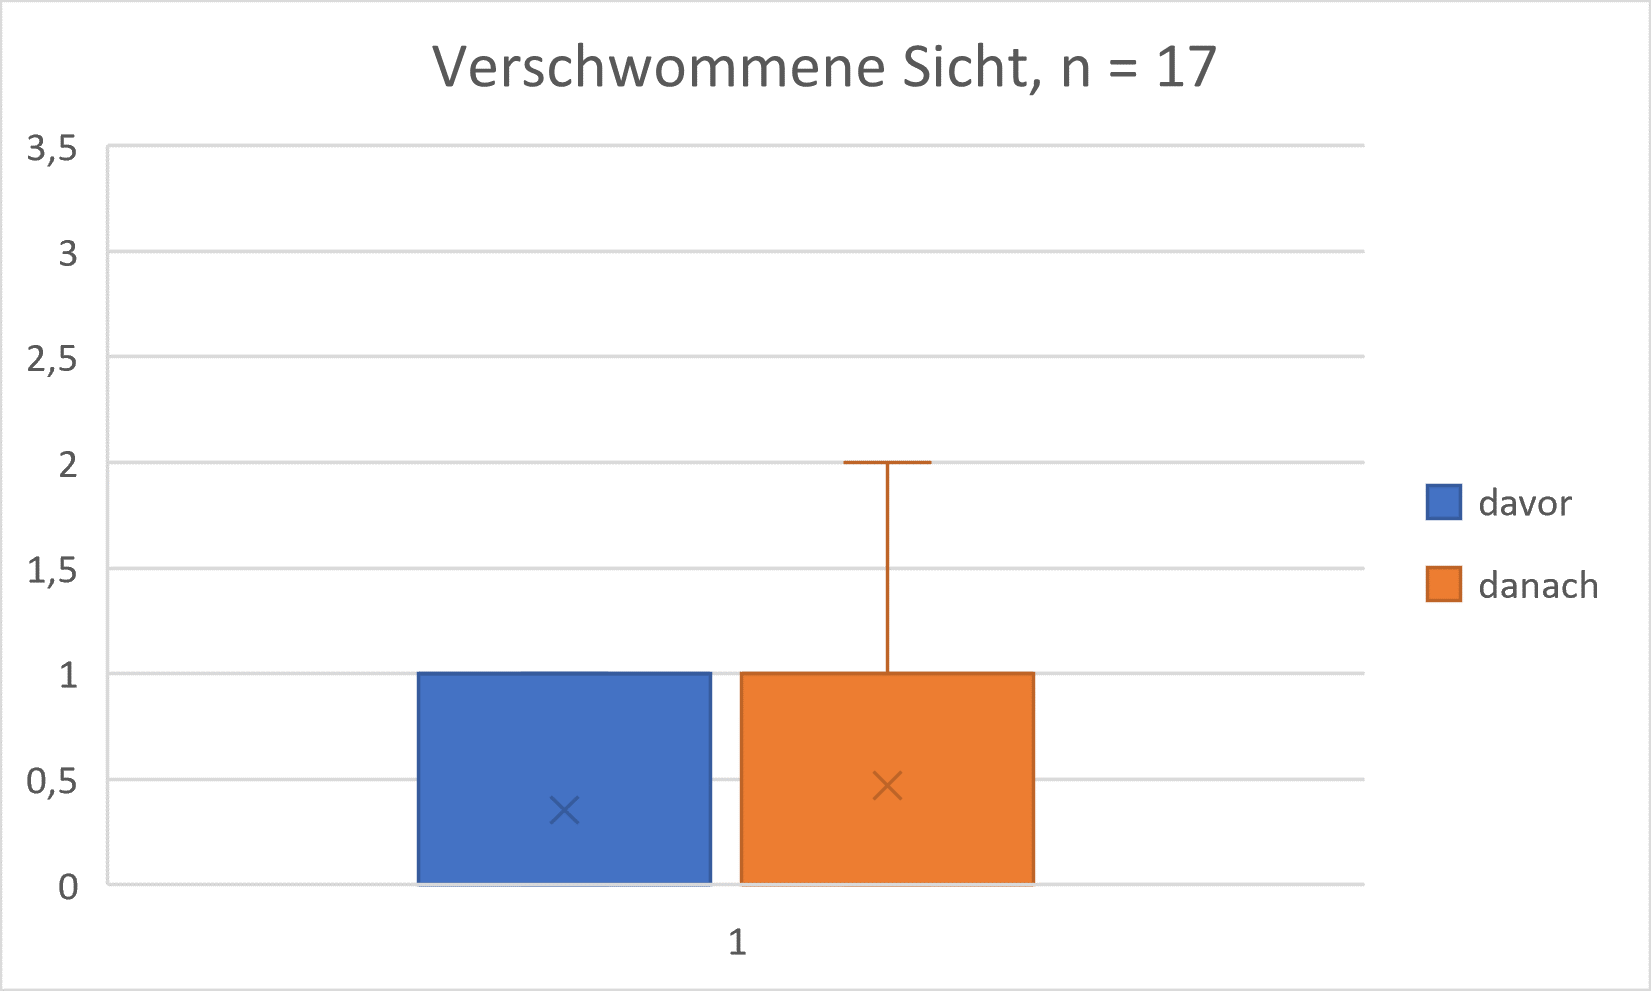
\includegraphics[width=0.2\textwidth]{assets/verschwSicht.png}
	\caption{Fragebogenergebnisse vorher nachher Vergleich}
	\label{fig:Fragebogenergebnisse}
\end{figure}
Lorem ipsum dolor sit amet, consetetur sadipscing elitr, sed diam nonumy eirmod tempor invidunt ut labore et dolore magna aliquyam erat, sed diam voluptua. At vero eos et accusam et justo duo dolores et ea rebum. Stet clita kasd gubergren, no sea takimata sanctus est Lorem ipsum dolor sit amet. Lorem ipsum dolor sit amet, consetetur sadipscing elitr, sed diam nonumy eirmod tempor invidunt ut labore et dolore magna aliquyam erat, sed diam voluptua. At vero eos et accusam et justo duo dolores et ea rebum. Stet clita kasd gubergren, no sea takimata sanctus est Lorem ipsum dolor sit amet.

Hier kommen noch mehr Ergebnisse rein...

\section{Diskussion}
\subsection{Limitationen}
Diese Einschränkungen sollten bei der Interpretation der Ergebnisse berücksichtigt werden:

\begin{myitemize}
	\item Unerfahrenheit mit EEG Technologie: Unser Team bestand aus fünf Studenten, die alle unerfahren im Umgang mit EEG-Technologien waren. Es wurde eine Einführung in das richtige Anlegen der Kappe, sowie Brille durchgeführt. Dennoch führte diese Unerfahrenheit zu Herausforderungen beim korrekten Anlegen der EEG-Elektroden bei einigen Probanden, insbesondere wenn diese bereits ein VR-Headset trugen. Dies könnte sich auf die Qualität der EEG-Signale ausgewirkt haben.
	\item Probandenauswahl: Die Anzahl der verfügbaren Probanden war begrenzt und es musste sicher gestellt werden, dass die ausgewählten Teilnehmer sowohl die erforderlichen Kriterien für unsere Forschungsfrage erfüllten als auch bereit waren, an den Probentests teilzunehmen.
	\item Stichprobengröße: Aufgrund der begrenzten Ressourcen und der Zeitbeschränkung konnte die Stichprobengröße nicht so groß sein, wie es für eine umfassendere Studie wünschenswert gewesen wäre. Eine größere Stichprobe hätte möglicherweise genauere und repräsentativere Ergebnisse erbracht.
	\item Beschränkungen der VR-Technologie: Bei Probanden mit kleineren Köpfen war es schwierig, das EEG richtig aufzusetzen, da das VR Headset zu viel Platz in der Stirnregion wegnahm. Dies beeinträchtigte möglicherweise die Platzierung der Elektroden und die Qualität der EEG-Signale.
	\item Mangelnde Erfahrung mit der verwendeten Software: Die Analyse der EEG-Daten erforderte den Einsatz spezifischer Software. Da innerhalb der Forschungsgruppe keine Erfahrung im Umgang mit der Analysesoftware bestand, musste zur Auswertung Recherche betrieben werden. Diese fehlende Erfahrung verlangsamte den Analyseprozess und erhöht das Potenzial für Fehler.
    \item Einschränkungen in Bezug auf Qualifikation und Expertise:
    Obwohl das Studienteam den Nutzertest erfolgreich durchgeführt und wertvolle Daten gesammelt hat, muss hervorgehoben werden, dass sich die Interpretation der EEG-Ergebnisse außerhalb der Expertise des Teams befindet. Da das Team aus keiner ausgebildeten medizinischen oder neurowissenschaftlichen Fachkraft besteht, fehlt das notwendige Wissen, um neurologische Daten präzise zu interpretieren und verlässliche Schlussfolgerungen daraus zu ziehen. Die Analyse kann daher nur auf oberflächliche Beobachtungen und allgemeine Trends in den Daten eingehen.

    In zukünftigen Studien, in denen neurologische Daten ausgewertet werden sollen, ist es von entscheidender Bedeutung, die richtige Testumgebung zu gewährleisten und die Zusammenarbeit mit qualifizierten Fachleuten in den Bereichen Neurologie und Datenanalyse sicherzustellen. Dies würde es ermöglichen, die gesammelten Daten vollständig zu nutzen und fundierte, wissenschaftliche Schlussfolgerungen zu ziehen. 
    
    Diese Einschränkung in Bezug auf die Qualifikation sollte nicht als Entschuldigung für ungenaue Ergebnisse angesehen werden, sondern vielmehr als Anreiz für zukünftige Projekte, bei denen eine interdisziplinäre Zusammenarbeit zur Maximierung der Qualität und Aussagekraft der Forschung angestrebt wird.

    Nichtsdestotrotz stellen diese Informationen eine wertvolle Ressource dar, die von qualifizierten Fachleuten in zukünftigen Projekten genutzt werden kann. Sie können als Vergleichsbasis dienen und dazu beitragen, Trends, Muster oder Abweichungen in ähnlichen Studien zu identifizieren. Dies unterstreicht die Bedeutung der Datenerfassung und -aufbewahrung, auch wenn die sofortige Analyse und Interpretation der Daten nicht möglich ist. Es wird empfohlen, zukünftige Teams und Fachleute zu ermutigen, diese Daten in ihrer Arbeit zu berücksichtigen und weiter zu erforschen.

    In zukünftigen Studien, in denen neurologische Daten ausgewertet werden sollen, ist es von entscheidender Bedeutung, die richtige Testumgebung zu gewährleisten und die Zusammenarbeit mit qualifizierten Fachleuten in den Bereichen Neurologie und Datenanalyse sicherzustellen. Dies würde es ermöglichen, die gesammelten Daten vollständig zu nutzen und fundierte, wissenschaftliche Schlussfolgerungen zu ziehen.

    Diese Einschränkung in Bezug auf die Qualifikation sollte nicht als Entschuldigung für ungenaue Ergebnisse angesehen werden, sondern vielmehr als Anreiz für zukünftige Projekte, bei denen eine interdisziplinäre Zusammenarbeit zur Maximierung der Qualität und Aussagekraft der Forschung angestrebt wird.

    Nichtsdestotrotz stellen diese Informationen eine wertvolle Ressource dar, die von qualifizierten Fachleuten in zukünftigen Projekten genutzt werden kann. Sie können als Vergleichsbasis dienen und dazu beitragen, Trends, Muster oder Abweichungen in ähnlichen Studien zu identifizieren. Dies unterstreicht die Bedeutung der Datenerfassung und -aufbewahrung, auch wenn die sofortige Analyse und Interpretation der Daten nicht möglich ist. Es wird empfohlen, zukünftige Teams und Fachleute zu ermutigen, diese Daten in ihrer Arbeit zu berücksichtigen und weiter zu erforschen.

    Es wird empfohlen, dass zukünftige Studien diese Einschränkungen berücksichtigen und gegebenenfalls weitere Untersuchungen durchführen, um die Auswirkungen dieser Faktoren auf die Ergebnisse zur Erkennung von potentiellem Stress durch den Akkomodations-Vergenz Konflikt zu minimieren.
\end{myitemize}

\subsection{Analyse}
Für die Analyse der Daten werden folgende Bandbreiten der EEG-Wellen betrachtet:
\begin{myitemize}
    \item Delta-Wellen (0,5 - 4 Hz): Diese sind oft während des tiefen Schlafes dominant.
    \item Theta-Wellen (4 - 8 Hz): Diese sind oft dominant in Zuständen tiefer Entspannung und Meditation.
    \item Alpha-Wellen (8 - 12 Hz): Diese sind oft dominant in Zuständen ruhiger Wachheit.
    \item Beta-Wellen (12 - 30 Hz): Diese sind oft dominant, wenn aktiv gedacht oder sich konzentriert wird.
    \item Gamma-Wellen (30 - 100 Hz): Diese werden oft mit hoher geistiger Aktivität und Informationsverarbeitung assoziiert.
\end{myitemize}

Die Analyse unterscheidet zudem drei Intervalle, die sich auf die Entfernung des zu fokussierenden Objekts beziehen:

\begin{myitemize}
    \item Erstes Intervall: Das Objekt bewegt sich vom Start (ca. 28 Meter) bis auf eine Entfernung von 1,5 Metern, was einer Dauer von drei Minuten entspricht. Hierbei ist zu beachten, dass die Startposition eine minimale Differenz aufweisen kann, da sich jeder Proband individuell bewegt und positioniert hat. Die Differenz beträgt nur wenige Zentimeter.
    \item Zweites Intervall: Das Objekt befindet sich in einer Entfernung zwischen 1,5 und 0,3 Metern, was einer Dauer von acht Sekunden entspricht.
    \item Drittes Intervall: Das Objekt befindet sich in einer Entfernung zwischen 0,3 und 0,15 Metern, was einer Dauer von etwa 15 bis 24 Sekunden entspricht.
\end{myitemize}

Die Analyse der Daten beschränkt sich hierbei auf die Beschreibung von Auffälligkeiten innerhalb der gemessenen EEG Daten in Form einer FFT (Fast Fourier Transform) und einem 3D-Mapping von sowohl der gesamten Gehirnwellen Typen als auch der einzelnen Typen im Verhältnis zu unseren 3 Zeitintervallen. Stichprobenhaft wurden dafür 5 Datensätze aus den 17 Probandentests ausgewählt. 


\subsection{Beschreibung}
Hier kommen die BEschreibungen der 5 3D-Maps rein plus die T-Test und die Box-Plots von Lukas und Patrick

\begin{thebibliography}{00}
\bibitem{b1} J. Frey, L. Pommereau, F. Lotte und M. Hachet, 'Assessing the zone of comfort in stereoscopic displays using EEG', ACM SIGCHI Conference on Human Factors in Computing Systems (S. 2041–2046. doi: 10.1145/2559206.2581191. [Online]. Verfügbar unter: https://arxiv.org/pdf/1404.6222)

\bibitem{b2} Statista. Virtual Reality - 'Prognose zum Umsatz weltweit bis 2026' | Statista. https://de.statista.com/statistik/daten/studie/318536/umfrage/prognose-zum-umsatz-mit-virtual-reality-weltweit/ (Zugriff am: 6. Juni 2023).

\bibitem{b3} A. Tatnall, Encyclopedia of education and information technologies. SPRINGER, 2020.

\bibitem{b4} U. Schmidt, Professionelle Videotechnik: Grundlagen, Filmtechnik, Fernsehtechnik (S. 27-28), Geräte- und Studiotechnik in SD, HD, DI, 3D, 6. Aufl. Berlin, Heidelberg: Springer Berlin Heidelberg; Imprint: Springer Vieweg, 2013.

\bibitem{b5} M. Guo, Y. Liu, B. Zou und Y. Wang, 'Study of electroencephalography-based objective stereoscopic visual fatigue evaluation,' in 2015 International Symposium on Bioelectronics and Bioinformatics (ISBB), 2015, S. 160–163, doi: 10.1109/ISBB.2015.7344948.

\bibitem{b6} P. Geraedts, Motorische Entwicklung und Steuerung: Eine Einführung für Physiotherapeuten, Ergotherapeuten und Trainer, 1. Aufl. Berlin, Germany: SPRINGER, 2020, S. 154-155.

\bibitem{b7} Wilder Penfield und Theodore Rasmussen, The Cerebral Cortex of Man: A Clinical Study of Localization of Function. New York: The Macmillan Company, 1950, S. 22.

\bibitem{b8} Frings, Biologie der Sinne. Springer Berlin Heidelberg, 2019, S. 193.

\bibitem{b9}Wearable Sensing | Dry EEG. DSI-24. Zugegriffen 12. Juli 2023. https://wearablesensing.com/dsi-24/.
\bibitem{b10}BESA® | Brain Electrical Source Analysis: BESA Research > Besa Research 7.1. Zugegriffen 12. Juli 2023. https://www.besa.de/home/downloads/besa-research/besa-research-7-1/.
\bibitem{b11}The professional-grade VR headset | VIVE Pro Deutschland. Zugegriffen 12. Juli 2023. https://www.vive.com/de/product/vive-pro/.


\end{thebibliography}
\vspace{12pt}
\color{red}
IEEE conference templates contain guidance text for composing and formatting conference papers. Please ensure that all template text is removed from your conference paper prior to submission to the conference. Failure to remove the template text from your paper may result in your paper not being published.

\end{document}
